\documentclass[14pt,utf8x,hyperref={pdfpagelabels=false}]{beamer}

\usepackage[utf8]{inputenc} % hyperref broken with utf8x
\usepackage[C40,T1]{fontenc}

\usepackage{graphicx}

\usepackage[francais]{babel}

\usepackage{tikz, pgfplots}
\usepackage{tikz-qtree}
\usetikzlibrary{shapes.arrows,chains,positioning}

\usetheme{moulardthesis}


\title{Optimisation numérique\\
  Exécution~de~trajectoires référencées capteurs}
\author{Thomas Moulard}
\date{Lundi 17 septembre 2012}


% Setup pdf meta-data.
\hypersetup{
pdfauthor = {Thomas Moulard},
pdftitle = {Optimisation num\'erique pour la robotique%
 et ex\'ecution de trajectoires r\'ef\'erenc\'ees capteurs},
pdfsubject = {Optimisation num\'erique pour la robotique%
 et ex\'ecution de trajectoires r\'ef\'erenc\'ees capteurs},
pdfkeywords = {optimisation numérique, typage, type,%
robotique, humano\"ide},
pdfcreator = {Thomas Moulard},
pdfproducer = {Thomas Moulard}
}


\begin{document}

{
  \usebackgroundtemplate{%
    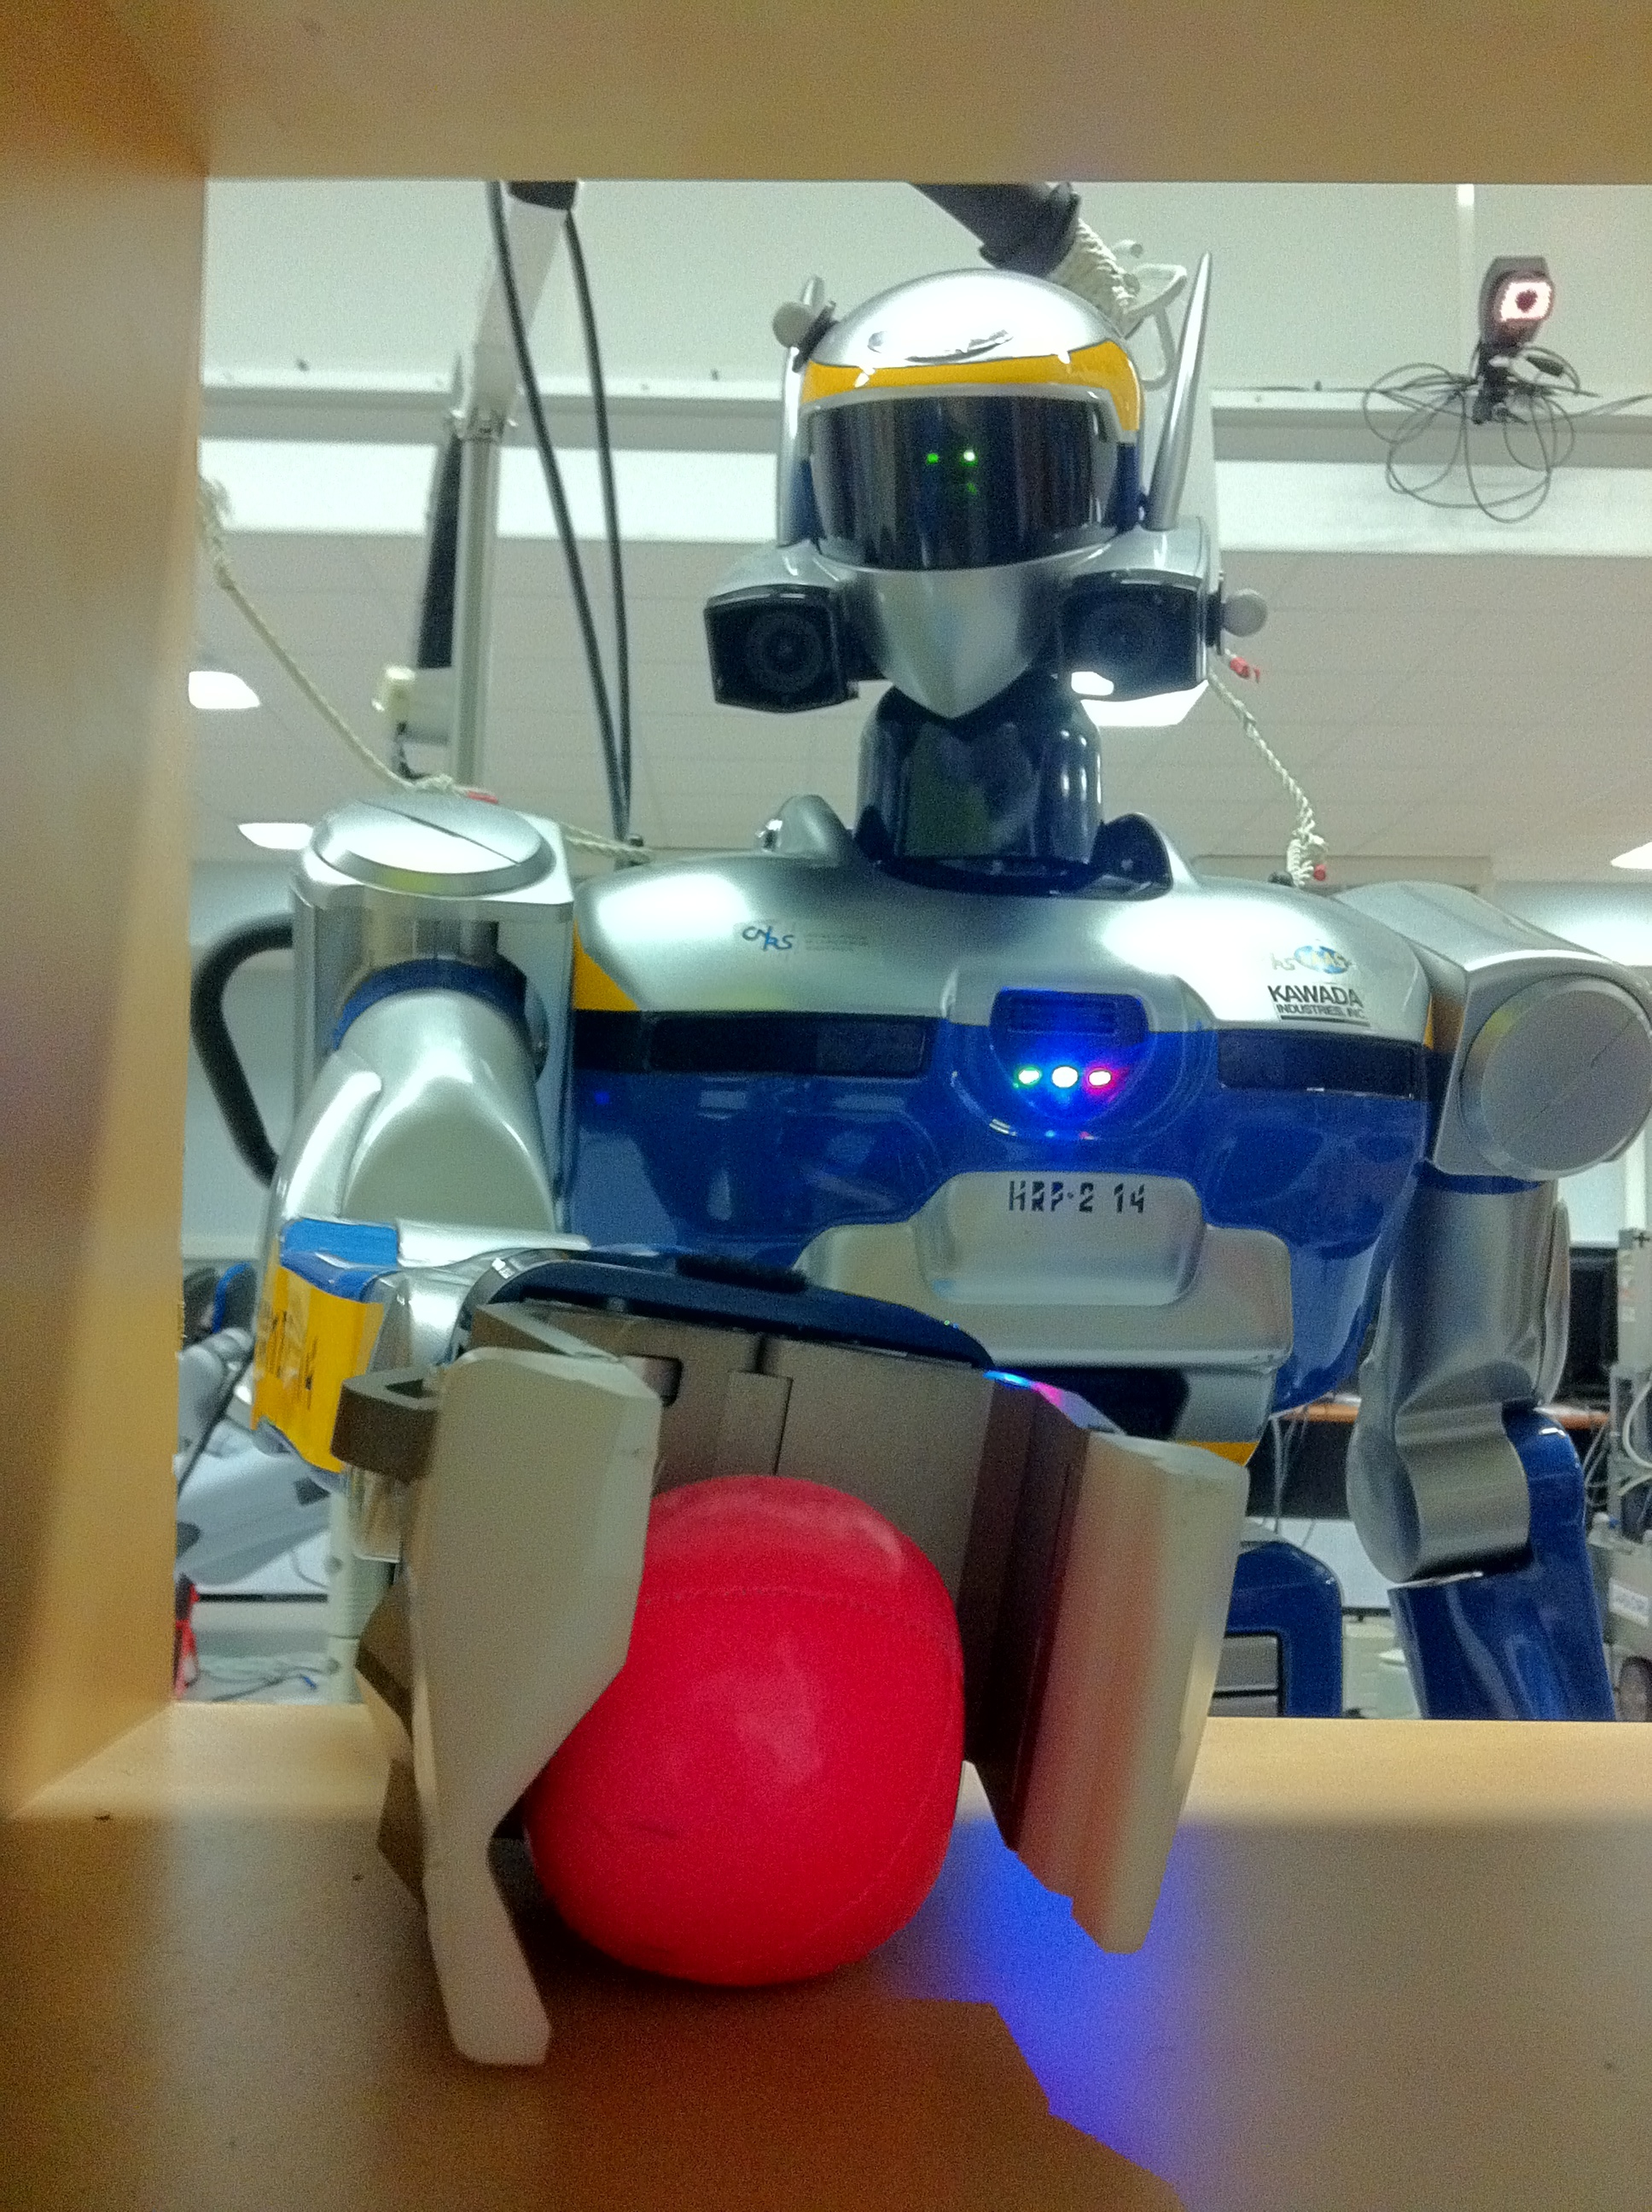
\includegraphics[width=\paperwidth,height=\paperheight]{%
      src/slides/demo1.jpg}}
  \begin{frame}[plain]
    \titlepage
  \end{frame}
}

%\maxFrameImage{src/slides/demo1.jpg}
%\maxFrameImage{src/slides/demo2.jpg}

% Introduction
% Animated scheme introducing contributions.
\begin{frame}[plain]
  \begin{changemargin}{-1cm}{-1cm}
    \begin{center}
      \tikzstyle{normalPath} = [line width=.7mm, color=black!50, -latex]

      \begin{tikzpicture}[
          auto,
          state/.style={
            rectangle,
            minimum size=6mm
          }]

        \uncover<1->{
          \node (perception) [state] {%
            
\includegraphics[height=3cm]{%
              src/slides/perception.jpg}};
        }

        \uncover<1>{
          \node (perception-description)
                [state, right=of perception]
                {\textbf{Perception}};
        }


        \uncover<2->{
          \node (decision)
               [state,above right=of perception] {%
            
\includegraphics[height=3cm]{%
              src/slides/decision.jpg}};
        }

        \uncover<2>{
          \node (decision-description)
                [state, right=of decision]
                {\textbf{Décision}};
        }

        \uncover<3->{
        \node (action) [state,below right=of decision]{%
          
\includegraphics[height=3cm]{%
            src/slides/action.jpg}};
        }

        \uncover<3>{
          \node (action-description)
                [state, left=of action]
                {\textbf{Action}};
        }

        \uncover<4->{
          \path (perception) edge[->, normalPath] (decision);
        }
        
        \uncover<5->{
          \path (decision) edge[->, normalPath] (action);
        }
        
        \uncover<6->{
          \path (action.south)
          edge[->, normalPath, dashed, bend right, bend left]
          node[color=black!50,above=5pt] {Monde réel}
          (perception.south);
        }

        \uncover<7->{
          \node (contrib) [state,left=of decision]{%
            \usebeamerfont{section}\large\textbf{Contributions}};

          \node (contrib1b) [state,right=1pt of decision]{%
            (1) RobOptim};
        }
        \uncover<7>{
          \node[thick,draw=ThoughfulBrick] (contrib1)
               [state,above=-3.4cm of decision] {%
                 \phantom{
\includegraphics[height=3.5cm]{%
                     src/slides/perception.jpg}}};
        }

        \uncover<8->{
          \path (perception.east)
          edge[->, normalPath,color=ThoughfulBrick]
          node[above=5pt] {(2) Correction}
          (action.west);
        }
        \uncover<8>{
          \node[thick,draw=ThoughfulBrick] (contrib2)
               [state,above=-3.4cm of action] {%
                 \phantom{
\includegraphics[height=3.5cm]{%
                     src/slides/action.jpg}}};
        }

%FIXME ajouter primitive mouvement ici

        \uncover<9->{
          \node (contrib3b) [state,above=10pt of perception]{%
            (3) Intégration};
        }
        \uncover<9>{
          \node[thick,draw=ThoughfulBrick] (contrib4)
               [state,above=-3.4cm of perception] {%
                 \phantom{
\includegraphics[height=3.5cm]{%
                     src/slides/perception.jpg}}};
        }


      \end{tikzpicture}
    \end{center}
  \end{changemargin}
\end{frame}

\section{Optimisation numérique pour la robotique}

{
  \usebackgroundtemplate{%
    \vspace{-2cm}
    \hspace{-4cm}
    
\includegraphics[height=\paperheight]{%
      src/slides/perception.jpg}}
  \begin{frame}[plain]
    absence de strategie analytique, outil polyvalent
  \end{frame}
}


\begin{frame}
  \frametitle{Le typage au secours du roboticien}

  courte introduction au typage
\end{frame}

\begin{frame}
  \frametitle{État de l'Art}

  algorithmes et logiciels
\end{frame}

\begin{frame}
  \frametitle{Modélisation informatique proposée}

  theoremes
\end{frame}

\begin{frame}
  \frametitle{Applications}

  slide karim
\end{frame}


\section{Exécution de trajectoire en boucle fermée}

\begin{frame}
  \frametitle{La marche bipède}

  FIXME
\end{frame}

\begin{frame}
  \frametitle{Contrôleur polyvalent pour la robotique}

  FIXME
\end{frame}

\begin{frame}
  \frametitle{Schéma de contrôle boucle fermée}

  FIXME
\end{frame}

\begin{frame}
  \frametitle{Correction de la pile de pas}

  FIXME
\end{frame}

\begin{frame}
  \frametitle{Correction de la trajectoire des pieds}

  FIXME
\end{frame}

\begin{frame}
  \frametitle{Correction de la trajectoire du centre de masse}

  FIXME
\end{frame}


\begin{frame}
  \frametitle{Résultats expérimentaux}

  FIXME
\end{frame}


\section{Intégration}

\begin{frame}
  \frametitle{Du magnétophone au robot}

  FIXME
\end{frame}

\begin{frame}
  \frametitle{De la bibliothèque au composant}

  FIXME
\end{frame}

\begin{frame}
  \frametitle{Résultats}
  FIXME
\end{frame}


\begin{frame}
  CONCLUSION
\end{frame}


\end{document}
